\cleardoublepage
\chapter{Estado del arte}


En este capítulo se describen el estado del ámbito del proyecto y de las tecnologías utilizadas para la realización del mismo.


\section{Mining Software Repositories}

Este Proyecto de Fin de Carrera, puede asociarse al área de los Mining Software Repositories -MSR-. El objetivo de la comunidad MSR es aprovechar todos los datos que se generan en el proceso de desarrollo software.


En general, estos datos se hallan en repositorios de software, como por ejemplo repositorios de control de cambios del código fuente -como Git-, repositorios de seguimiento de bugs y errores, o repositorios de comunicaciones que almacenan las comunicaciones entre el equipo de desarrolladores como es el caso de las listas de distribución. \\

La comunidad MSR se dedica a encontrar fuentes de información provenientes de los proyectos software, estudiar sus características, encontrar técnicas para extraer de forma efectiva la información y el aprovechamiento de esos datos para mejorar los requisitos, la calidad y la trazabilidad de los proyectos, y estudiar el impacto de diferentes fenómenos en un desarrollo.


Gran parte del conocimiento y evolución en este campo, se presenta anualmente en la conferencia de MSR, cuya décimo cuarta edición se ha celebrado este año en Buenos Aires, conjuntamente a la Conferencia Internacional de Ingeniería de Software.


En esta conferencia, se presentan los artículos sobre MSR que han sido aceptados tras su revisión y entre las actividades se encuentra la propuesta de un desafío sobre un conjunto de datos propuesto, para el cual los que aceptan ser desafiados tienen que solucionar a través de sus herramientas o sistemas MSR y presentar un reporte de los resultados.


Las temáticas dentro de los MSR, entre muchas otras, podemos enumerar, por ejemplo:

\begin{itemize}
\item Predicción de las características del software mediante el análisis del repositorio software.

\item Caracterización, clasificación y predicción de defectos en el software mediante el análisis de los repositorios software.

\item Análisis de cambios o de nuevas tendencias.

\item Técnicas de visualización y modelos para los conjuntos de datos minados.

\item Privacidad y ética en los MSR.

\item Minado sobre cualquier elemento asociado a un proceso de desarrollo software. Los ya mencionados, pero también otros como licencias, \textit{logs} o las opiniones en los centros de aplicaciones y sitios de opiniones sobre los programas.
\end{itemize}


Centrándose más en la parcela relativa a este proyecto. Por otra parte, las experiencias piloto que suponen el punto de partida de este Proyecto de Fin de Carrera, fueron analizadas y expuestas en \textit{Gregorio Robles y Jesús M. González-Barahona (2013). Mining student repositories to gain learning analytics}. En éste, se expone el proceso de corrección, que ya describimos en el capítulo 2. 

Entre las conclusiones del articulo, se expone que proporciona importantes beneficios al facilitar la evaluación continua y realimentación frecuente a los alumnos. El otro hecho que se concluye, es que un sistema de estas características, que se ha tenido que refinar en un proceso iterativo, no es posible hacerse completamente automático, y se deben tomar medidas para minimizar las tareas manuales del proceso, la principal, es que los estudiantes sigan estrictamente las instrucciones indicadas para la realización de la actividad.


Asimismo, a la hora de explorar formas y herramientas para explotar los datos brutos de las entregas de los alumnos, me resultó útil a nivel conceptual el análisis de las diferentes fuentes que nos podemos encontrar en un proyecto de software, que se realiza en el artículo \textit{Robles, G., González-Barahona J. M., Izquierdo-Cortazar, D. y Herraiz, I. (2009). Tools for the Study of the Usual Data Sources found in Libre Software Projects}.


\section{Tecnologías utilizadass} 
\label{sec:tec_use}

\subsection{Python} 
\label{sec:python}


Python es un lenguaje de programación interpretado, usa tipado dinámico y es multiplataforma. Además se trata de un lenguanje de programación multiparadigma, permitiendo programación orientada a objetos, imperativa y funcional. Además posee una extensa biblioteca estándar y existen infinidad de librerías de terceros.


Dadas sus características, Python es muy útil como lenguaje para scripting y desarrollo rápido de aplicaciones de todo tipo.


Esta licenciado bajo la \textit{Python Software Foundation License} desde la versión 2.1, licencia declarada libre, y compatible con GPL.


Fue creado por Guido van Rossum -el Benevolente Dictador Vitalicio- en los Países Bajos a finales de los años 80 y su nombre proviene de los humoristas británicos Monty Python.


La versión 1.0 fue lanzada en 1994, la 2.0 en Octubre de 2000 y la 3.0 fue lanzada en Diciembre de 2008. Actualmente, coexisten dos versiones de Python, la 2 y la 3, con diferencias que las hacen incompatibles, siendo las últimas versiones la 3.6.1 y la 2.7.13.


Python pretende ser un lenguaje fácil de leer. Para delimitar bloques se emplea la indentación en blancos en lugar de las llaves y los puntos y coma. En el mundillo Python, existe una filosofía  con unos principios de Python en cuenta a legibilidad y transparencia, recogida en el documento ``El Zen de Python'' (PEP 20). El código que siga sus principios se denomina \textit{pythonic}.


\subsection{Django} 
\label{sec:django}


Django es un framework de aplicaciones web open source, escrito en Python, que aparenta seguir el patrón de diseño Modelo-Vista-Controlador. Proporciona al usuario una serie de componentes habituales en las aplicaciones web, como autenticación, sesión, administración, formularios, gestión de archivos, ya preparados para ser usados.


Está orientado a realizar desarrollos rápidos, por lo que incluye un servidor web ligero para facilitar esto, aunque soporta \textit{Apache2} para la etapa de producción y servidores \textit{WSGI}. Las bases de datos soportadas son \textit{PostgreSQL}, \textit{MySQL} y \textit{SQLite3}.


Django fue liberado al público bajo licencia BSD en 2005, siendo desde 2008 la \textit{Django Software Foundation} quien mantiene el proyecto. La última versión es la 1.11, que será la última que soporte Python 2.


\subsection{MongoDB} 
\label{sec:mongodb}


MongoDB es un sistema de base de datos NoSQL lanzado en 2009 y ampliamente adoptado por la industria. La última versión es la 3.4.4. Es orientado a documentos, los cuales se guardan en colecciones de documentos de una estructura similar a JSON -BSON-.  La equivalencia entre elementos de una BBDD SQL y NoSQL, es la siguiente:

\begin{itemize}
\item Tabla - Colección

\item Registro - Documento

\item Columna - Campo
\end{itemize}


Hace uso de esquemas dinámicos y no existe un esquema predefinido, pudiéndose alterar en cualquier momento, e incluso tener una misma colección varios documentos con distintos campos. Es un paradigma muy válido y eficaz en aplicaciones que necesiten almacenar datos semi-estructurados y facilitan los procesos de desarrollo iterativo.


No es recomendable para aplicaciones que usen intensivamente \textit{JOINS} o requieran transacciones en lugar del bloqueo a nivel de documento que realiza MongoDB. Asimismo, puede presentar problemas de consistencia entre documentos, las escrituras no son verificables y puede perderse información.


MongoDB viene por defecto con una consola construida sobre Javascript, realizándose las consultas y operaciones en este lenguaje, y pudiéndose usar la sintaxis elemental de este lenguaje.


Asimismo, MongoDB tiene drivers oficiales para los principales lenguajes de programación. Para Python, el driver recomendado es PyMongo.


\subsubsection{PyMODM} 
\label{sec:pymod}

PyMODM, es un ODM sobre el driver de MongoDB PyMongo, desarrollado por ingenieros de MongoDB. Es una librería que proporciona los mecanismos para mapear la estructura de la base de datos a objetos Python, pudiéndose usar la información de la base de datos como si se tratase de un objeto.


\subsection{GIT} 
\label{sec:git}

Git es un sistema de control de versiones de software libre, diseñado por Linus Torvalds y lanzado en 2005. Se caracteriza por ser una herramienta distribuida, muy eficiente de proyectos grandes y que soporta muy bien el desarrollo no lineal en un proyecto, con la gestión de ramas, diferencias y mezclado de versiones.


En Git, los datos se modelan y almacenan como una sucesión de instantáneas de un pequeño sistema de archivos cada una, salvo el caso de ficheros idénticos entre dos instantáneas, que se referencian mediante un link. Además, todos los objetos en git son verificados mediante SHA-1 a bajo nivel, por lo que Git posee integridad.


Para operar con el repositorio o el historial, no es necesario  estar conectado al servidor, salvo para sincronizar los cambios, pudiendo operar todo el tiempo en local.


\subsubsection{PyGIT2} 
\label{sec:pygit2}

Librería externa de Python, que proporciona en Python la funcionalidad esencial de Git a través de \textit{Libgit2}, la API en C multiplataforma.

\subsection{Análisis de código fuente} 
\label{sec:anal_cod}

El análisis del código fuente, es un tipo de análisis dentro del análisis estático de software, habitualmente realizado por herramientas automáticas, que evalúa el software sin ejecutarlo, para permitir mejorar el código, sin alterar la semántica.


En un análisis estático de código automático, se incluyen análisis de sintáxis del código fuente, y diferentes reglas a aplicar sobre determinadas estructuras de código.


En el caso del análisis humano, este se denomina comprensión de programas o también revisión de código, que es complementario al automático y permite evaluar aspectos que un sistema automático no suele cubrir, como la arquitectura, el diseño, o la forma de trabajar con elementos externos.


Los objetivos de estos análisis puede ser tales como la verificación de propiedades del software para seguridad, detección de código vulnerable, la mejora de la calidad, o mejorar el mantenimiento y desarrollo.


No obstante, el análisis de código fuente no es suficiente para evaluar o mejorar un desarrollo en todos sus aspectos, por lo que debería complementarse con otras técnicas de análisis de software, por ejemplo, los test.


\subsubsection{UTILIDADES DE ANÁLISIS DE CÓDIGO FUENTE EN PYTHON} 
\label{sec:utilidades_cod}


Para la realización de análisis de código en Python, nos hemos ayudado de varias herramientas, introducidas a continuación.


La utilidad Pep8, que recientemente se ha rebautizado como \textit{Pycodestyle}, es un \textit{checker} de la guía de estilo de Python. Esta utilidad, se ejecuta sobre ficheros fuente Python, y nos proporciona un listado con la localización, el código de error E*** o W*** y la descripción de los incumplimientos con respecto a la guía de PEP8.


Pylint, es otra utilidad de verificación de código Python bastante completa, que verifica estilo, bugs y calidad del código. También si los nombres de los elementos están bien formados con respecto a los estándares y si las interfaces declaradas son implementadas. Es una herramienta comúnmente integrada en los entornos de desarrollo y editores de código.


Flake8 es una utilidad que auna las comprobaciones de estilo de Pep8, de errores de lógica de Pyflakes, y de complejidad circular. Su diseño permite la extensión mediante la inclusión de extensiones. Por defecto incluye la extensión McCabe, que generaría errores con el codigo C9**, si detecta casos de complejidades mayores a un umbral dado. Las comprobaciones de errores de lógica de Pyflakes se etiquetan mediante códigos F***.


Otra extensión popular es Hacking, que introduce errores con el código H***, y sus comprobaciones son las contempladas en \textit{OpenStack Style Guidelines}, basadas en  \textit{Google Python Style Guidelines}.

Existe una completa documentación de los códigos de error en los manuales de las diferentes utilidades mencionadas.


\section{Otras herramientas utilizadas} 
\label{sec:otras_herramientas}

El desarrollo de este proyecto se ha realizado eminentemente desde y para sistemas Linux, y concretamente se ha desarrollado y probado en distribuciones Ubuntu y Linux Mint, semejantes a los entornos que emplean profesores y alumnos en el contexto tratado.


En otros casos, aunque Python es un lenguaje multiplataforma y Misture emplea muchas librerias y utilidades que también lo son, inicialmente el desarrollo no esta considerado para otros sistemas, y exigiría la revisión de la totalidad de las dependencias de las librerías utilizadas. También sería necesaria la revisión y refactorización de algunos códigos, como por ejemplo  aquellos que emplean la librerías estándar \textit{os} y \textit{os.path}, para asegurar la plena independencia del código frente al sistema operativo.


Una vez circunscritos a estos sistemas, hay que recalcar que en general se ha intentado optar por el uso de editores, herramientas, librerías, DBMS de software libre, open source o en todo caso amigables con sus filosofías o licencias compatibles.


Aún así, durante el transcurso del proyecto, pasé a utilizar como IDE la herramienta Pycharm, que es privativa en su versión profesional, aunque contando con licencias especiales para proyectos de open source, y una versión básica con licencia no privativa.


En este caso, el cambio a este IDE viene justificado con una notable mejora de productividad ayudando a manejar la cantidad creciente de código, las ayudas y atajos para recordar y acceder a todas las librerías y APIs que he ido integrando, una gran ayuda en la detección de errores y \textit{warnings} previos a la ejecución, y en ejecución gracias a un potente debugger.


Una vez ya han sido introducidas con anterioridad las tecnologías, herramientas y librerías clave, paso a hacer una mención de dos de las herramientas que he conocido durante la realización de este proyecto, y que han sido de notable ayuda para su realización.

\subsection{PyCharm}
\label{subsec:pycharm}

Como ya se ha introducido, PyCharm es un IDE multiplataforma orientado al lenguaje Python, y también al desarrollo de JavaScript y soporte para \textit{frameworks} basados en estos lenguajes cono AngularJS o Django. Pycharm aporta además, entre otras funcionalidades:

\begin{itemize}
\item Ayuda y análisis de código: autocompletado, marcado de sintaxis y errores.

\item Navegación avanzada entre los elementos del proyecto y del código.

\item Refactorización del código Python.

\item Depurador integrado.

\item Integración para test unitarios en Python.

\item Integración con sistemas de control de versiones: Git, Mercurial, Subversión, CVS.

\item Extensiones y disponibilidad de una numerosa biblioteca para infinidad de propósitos.

\item También permite la integración de herramientas externas. Por ejemplo, en nuestro caso integramos \textit{Pep8} y pudiéndose chequear el estilo de cualquier módulo rápidamente.
\end{itemize}

Jetbrains, la empresa desarrolladora de este producto, lo pone a disposición de los usuarios bajo un modelo que puede considerarse \textit{fremium}. Tienen disponible una versión profesional, privativa, con todas las funcionalidades y extensiones. Pero también, proporcionan licencias especiales para proyectos open source no comerciales, cuyas condiciones podemos encontrar en \space \url{https://www.jetbrains.com/buy/opensource/}.


\begin{figure}[H]
   \centering
   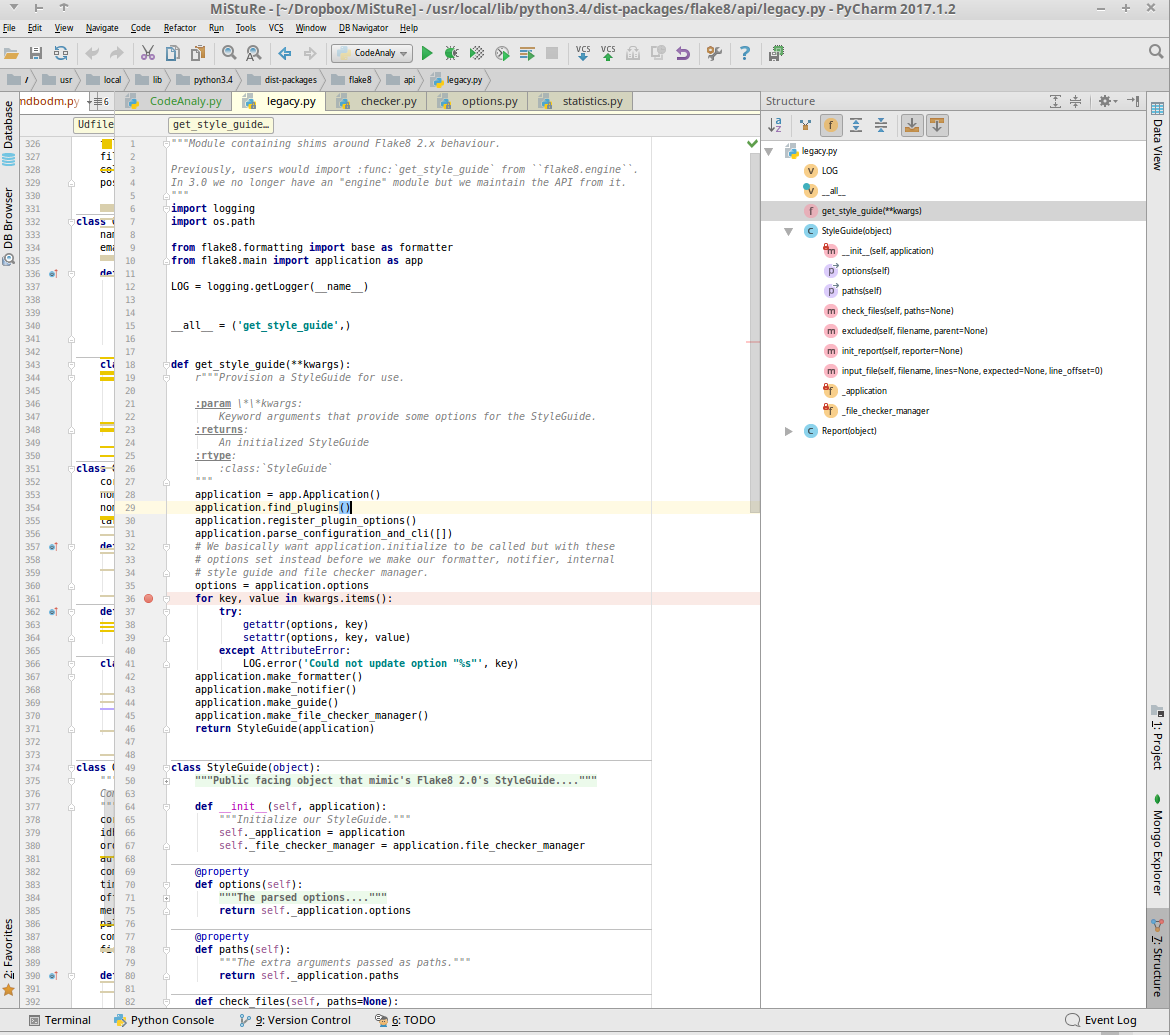
\includegraphics[width=16cm]{img/pycharm}
   \caption{Interfaz de PyCharm }
   \label{figura:pycharm}
\end{figure}



Asimismo, mantienen versiones básicas de sus productos lanzadas bajo licencias open source, como Apache 2.0, llegando a disponerse públicamente del código de algunos de ellos. Tal como es el caso de IntelliJ IDEA \space \url{https://github.com/JetBrains/intellij-community}, que es otro IDE desarrollado por ellos que es la propia base del IDE PyCharm.


En el caso de PyCharm, está versión es la denominada como ``Community Edition'', la cuál fue la que se empleo en el desarrollo y depuración de buena parte de este proyecto.




\subsection{Robomongo}
\label{subsec:robomongo}

Robomongo es un cliente para bases de datos MongoDB con interfaz gráfica, muy ligero y de funcionalidad básica, pero suficientemente potente.


Entre sus capacidades, integra la funcionalidad del cliente shell de MongoDB, permite la escritura de scripts y la vista de las propiedades, configuración y colecciones de las BBDD MongoDB del equipo. Resulta de gran ayuda navegación entre las diferentes colecciones y documentos y la posibilidad de visualizarlos en diferentes formatos como tabla, árbol, o la tradicional vista de texto en formato JSON.


\begin{figure}[H]
   \centering
   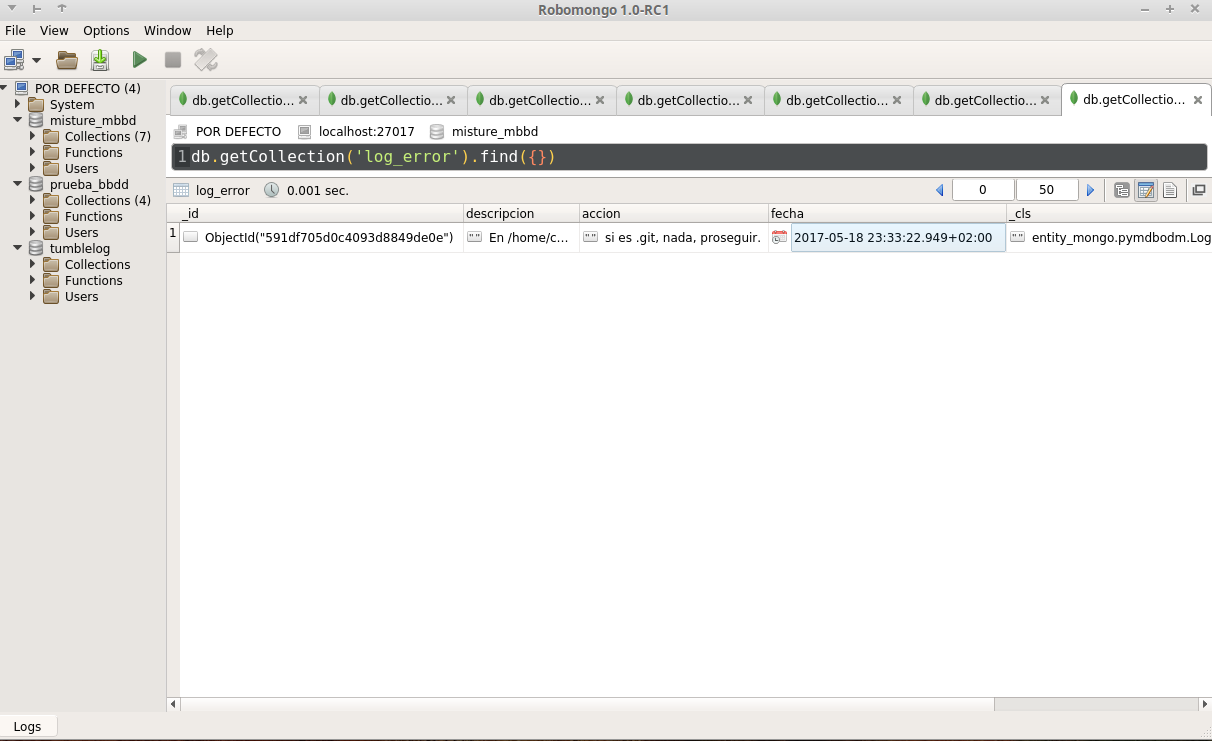
\includegraphics[width=16cm]{img/robomongo}
   \caption{Interfaz de Robomongo}
   \label{figura:robomongo}
\end{figure}


Robomongo era un proyecto open source cuyo código ha estado disponible públicamente. Recientemente, ha sido adquirido por la empresa Studio3T, que ha optado por mantener el proyecto en  open source \url{https://github.com/Studio3T/robomongo}, en paralelo a sus proyectos comerciales relativos a MongoDB.
